\begin{figure}
    \begin{center}
    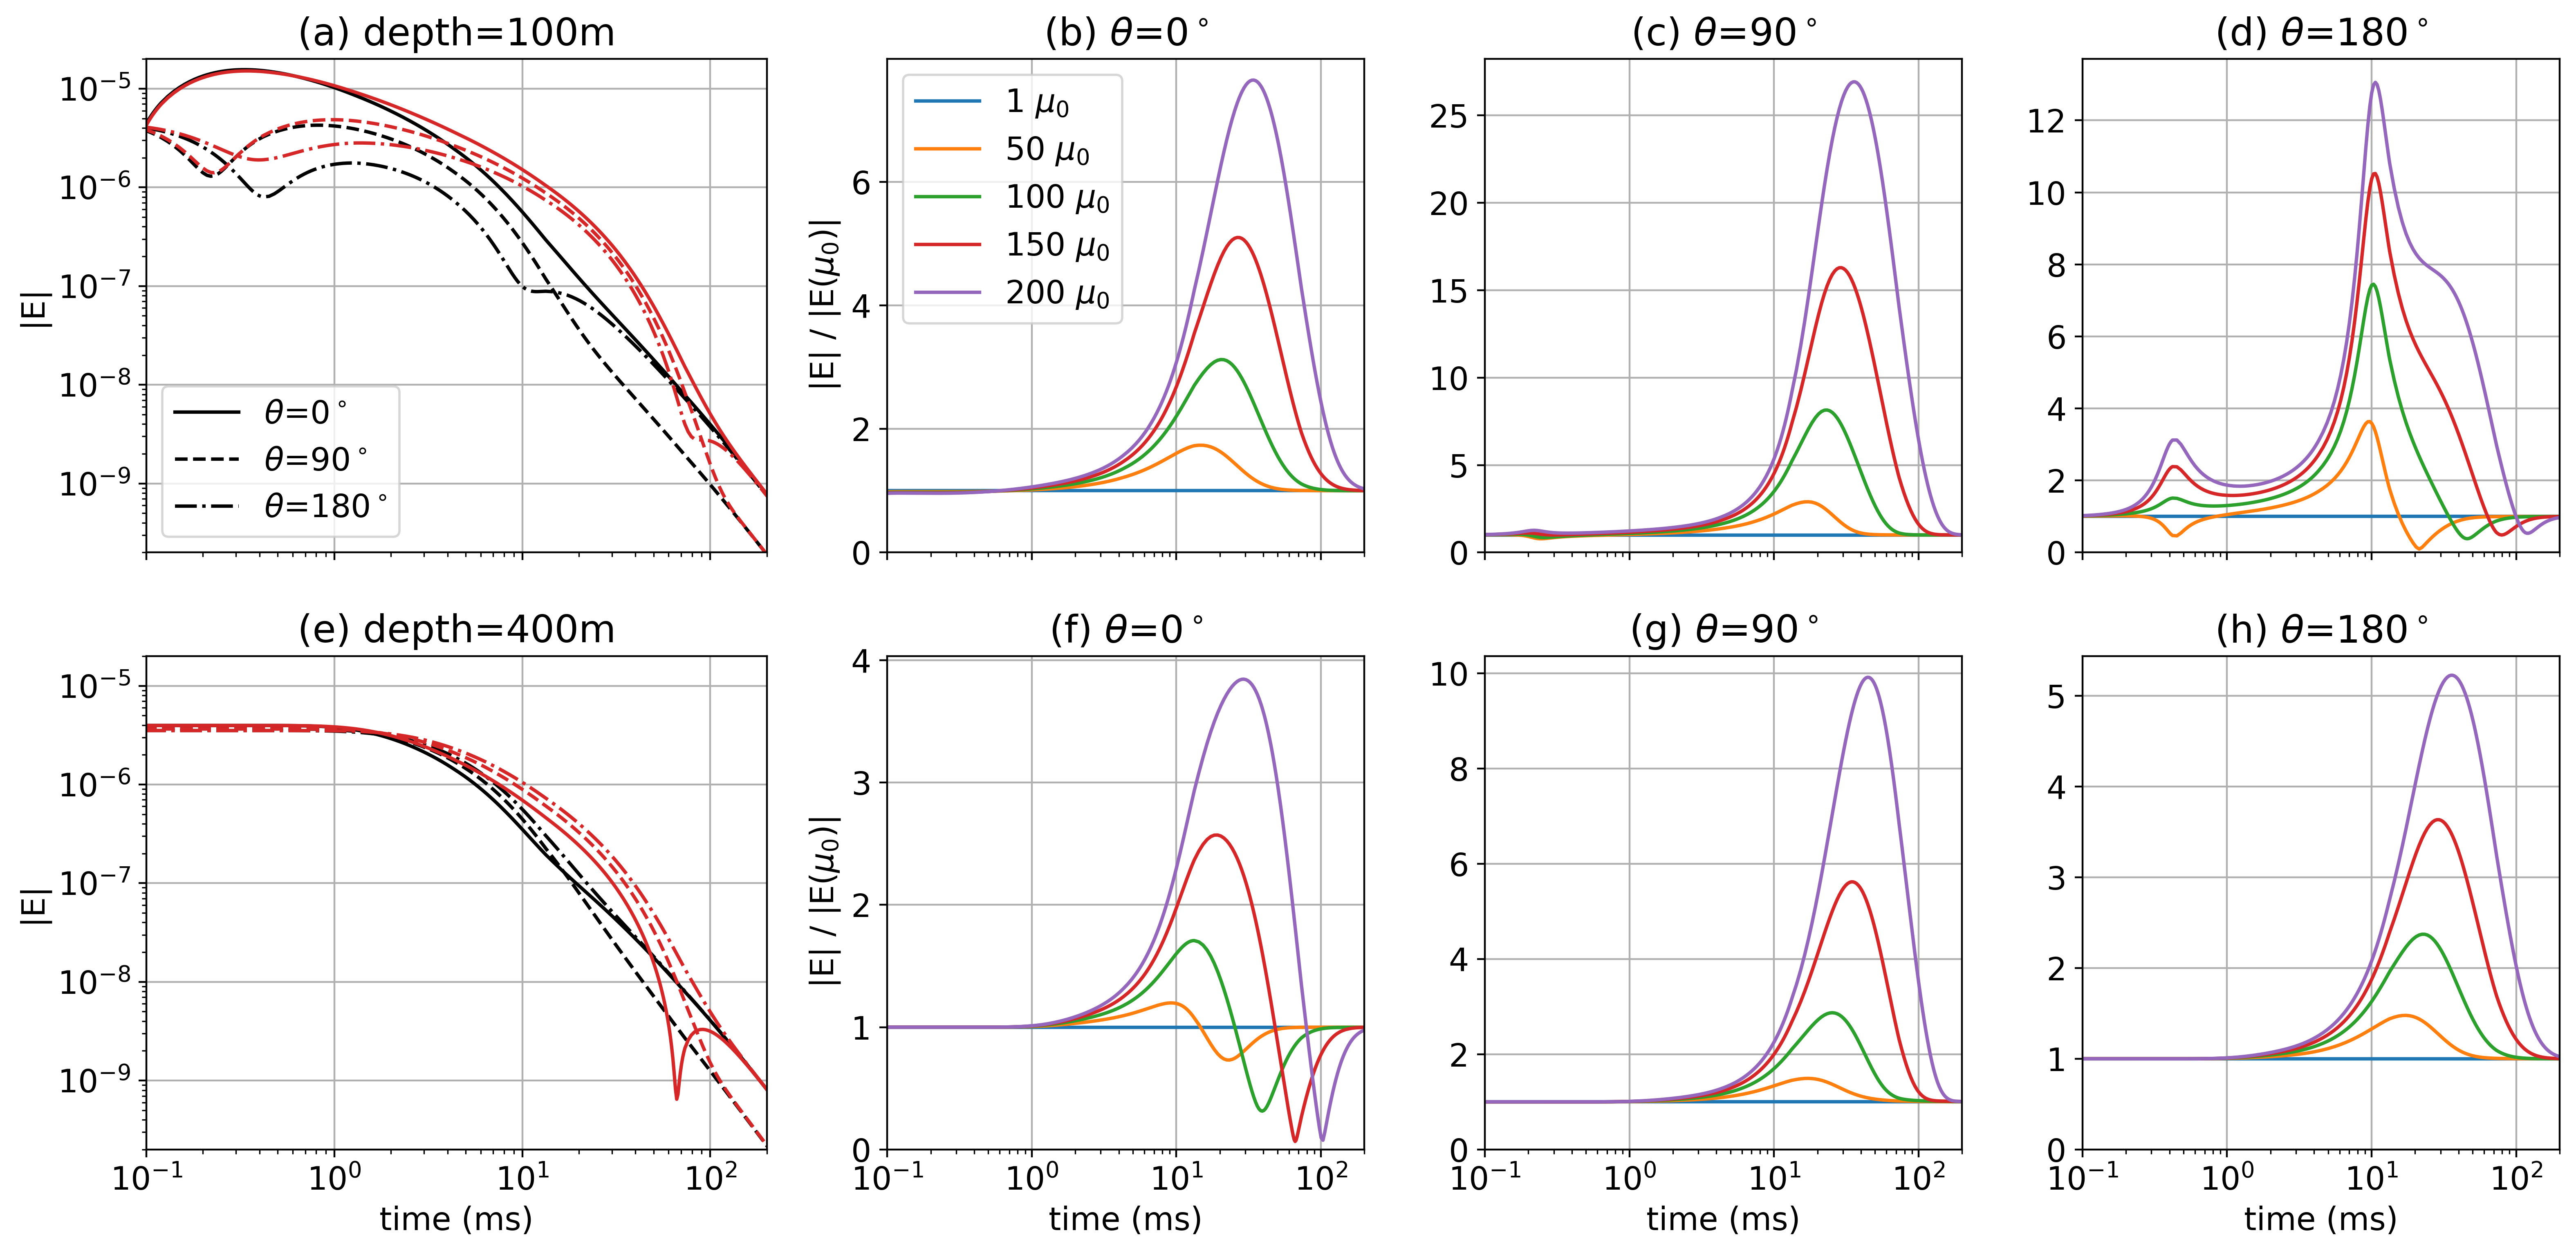
\includegraphics[width=\textwidth]{figures/excitation-time.png}
    \end{center}
\caption{
    Amplitude of the average electric field over a test volume that extends from 50m - 100m radially and 50m vertically centered about depths of (a) 100m and (e) 400m. The different line-styles in (a) and (e) indicate different azimuths ($0^\circ$ is under the transmitter wire, $90^\circ$ is orthogonal to it, and $180^\circ$ is opposite to it). The black line indicates the scenario for a well with permeability equal to that of free space $\mu_0$ and the red lines are for the scenario where the well has a permeability of $150\mu_0$. Panels (b), (c), and (d) show the ratio of the amplitude of the electric field with respect to the non-permeable well ($\mu=\mu_0$) for the test volume centered at a depth of 100m. Panels (f), (g) and (h) show the ratios of the electric field amplitude for the test volume centered at 400m depth.
}
\label{fig:excitation-time}
\end{figure}



